% Lab 1 report: Sieve of Eratosthenes in C++, Python and Julia.
% Build from lab1/:  pdflatex report.tex   (run twice for references)
\documentclass[11pt,a4paper]{article}

\usepackage[T1]{fontenc}
\usepackage[utf8]{inputenc}
\usepackage{lmodern}
\usepackage[margin=2.2cm]{geometry}
\usepackage{amsmath}
\usepackage{booktabs}
\usepackage{graphicx}
\usepackage{float}
\usepackage[hidelinks]{hyperref}

\newcommand{\code}[1]{\texttt{#1}}
\newcommand{\tenp}[1]{10^{#1}}

\title{Lab 1 report: Sieve of Eratosthenes in C++, Python and Julia}
\author{}
\date{October 5, 2026}

\begin{document}
\maketitle

\section{Experimental procedure}

\subsection*{Algorithm}
All implementations use the same full sieve. Each call allocates $N+1$ one-byte flags set to 1 and
clears the flags for 0 and 1. For each $p$ with $p \cdot p \le N$ whose flag is still 1, it clears
$p^2, p^2+p, \dots \le N$. It then counts the remaining 1-flags with a 64-bit accumulator and returns
only that count. Marking and counting use explicit loops. The flag array is filled in bulk. The
baseline uses no slicing, NumPy, \code{@inbounds}, \code{vector<bool>}, \code{BitArray} or
\code{unsafe}. The outer bound \code{p*p <= N} is equivalent to $p \le \lfloor\sqrt{N}\rfloor$ and
avoids rounding errors from a floating-point square root.

\subsection*{Correctness}
Before any timing, every program checks $\pi(N)$ for $N = 2, 10, 100, \tenp{5}, \tenp{6}$ and
$\tenp{7}$ against 1, 4, 25, 9\,592, 78\,498 and 664\,579. It also prints the surviving flags for
$N = 30$ (2 3 5 7 11 13 17 19 23 29). All five implementations passed. Every timed call in the CSV
returned the expected count.

\subsection*{Timing}
The timer starts immediately before \code{count\_primes(N)} and stops immediately after it returns.
The timed interval covers allocation, initialization, marking and counting. The count is stored and
printed after the timer stops. Printing, CSV output, checks and warm-up calls are outside the timed
interval. Timers: \code{steady\_clock} (C++), \code{perf\_counter} (Python), \code{time\_ns}
(Julia), \code{nanoTime} (Java), \code{Instant} (Rust). For each $N$, each program makes $W$ untimed
warm-up calls and then 10 timed calls in the same process. All runs used batch size 1. The shortest
call (C++, $N=\tenp{5}$, about 0.05\,ms) is still more than 1000 ticks of the $\approx$42\,ns macOS
clock.

\subsection*{Measurement blocks}
Block 1 used $W = 5$. Its Rust $N=\tenp{6}$ sequence trended downward, from 1.71 to 1.51\,ms, so I
repeated the complete measurement for all languages with $W = 20$ (block 2). Block 2 is the reported
block. Block 1 is kept in the CSV and marked \code{superseded}, and its medians appear in the last
column of Table~\ref{tab:results}.

\subsection*{Environment}
Apple M1 Pro, 16\,GB RAM, macOS 26.6.2, on battery with Low Power Mode off. Benchmarks ran one at a
time with no other heavy workload. Toolchains: Apple clang 21.0.0 with \code{-O3 -std=c++17},
CPython 3.14.2, Julia 1.13.1 (default options). The README lists the exact commands.

\section{Results}

Slowdown is the median divided by the smallest median among C++, Python and Julia at that $N$. C++
was the reference at every $N$.

\begin{table}[H]
\centering
\caption{Block 2 ($W = 20$, 10 timed calls each). Times in milliseconds.}
\label{tab:results}
\begin{tabular}{llrrrrrr}
\toprule
Language & $N$ & Median & Min & Max & $\pi(N)$ & Slowdown & Block-1 median \\
\midrule
C++    & $\tenp{5}$ & 0.0549 & 0.0547 & 0.0555 & 9,592   & 1.00  & 0.0380 \\
Python & $\tenp{5}$ & 8.48   & 8.43   & 8.87   & 9,592   & 154.7 & 8.39   \\
Julia  & $\tenp{5}$ & 0.0810 & 0.0796 & 0.0910 & 9,592   & 1.48  & 0.0817 \\
\midrule
C++    & $\tenp{6}$ & 0.835  & 0.834  & 0.946  & 78,498  & 1.00  & 0.716  \\
Python & $\tenp{6}$ & 90.7   & 90.4   & 91.5   & 78,498  & 108.7 & 90.0   \\
Julia  & $\tenp{6}$ & 1.06   & 1.02   & 1.21   & 78,498  & 1.27  & 0.992  \\
\midrule
C++    & $\tenp{7}$ & 9.38   & 9.24   & 10.09  & 664,579 & 1.00  & 10.91  \\
Python & $\tenp{7}$ & 953.5  & 948.2  & 958.2  & 664,579 & 101.7 & 949.4  \\
Julia  & $\tenp{7}$ & 11.42  & 11.14  & 12.01  & 664,579 & 1.22  & 11.01  \\
\bottomrule
\end{tabular}
\end{table}

\begin{figure}[H]
\centering
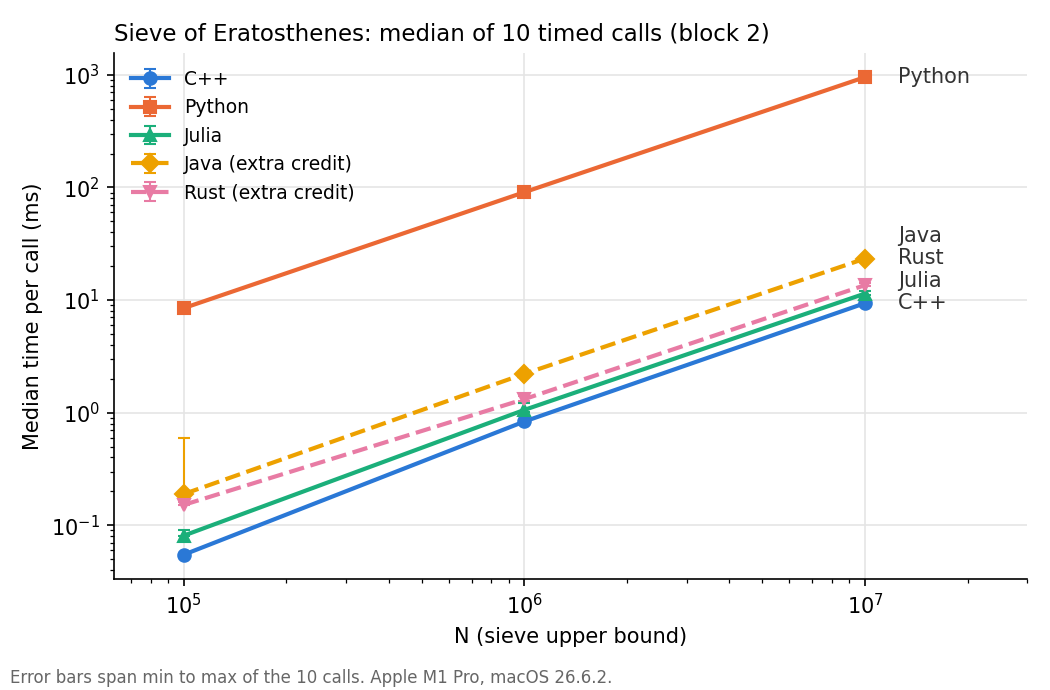
\includegraphics[width=0.85\textwidth]{results/scaling.png}
\caption{Median time per call against $N$ on log-log axes. Error bars run from the minimum to the
maximum of the 10 timed calls and are mostly smaller than the markers. The Java and Rust curves are
discussed in the appendix.}
\label{fig:scaling}
\end{figure}

\section{Analysis}

\subsection*{Q1. Fastest and slowest}
C++ had the lowest median at every $N$. Python had the highest median at every $N$: $155\times$,
$109\times$ and $102\times$ the C++ median at $\tenp{5}$, $\tenp{6}$ and $\tenp{7}$. This gap is two
orders of magnitude larger than any spread I observed, so the result is convincing. The C++ vs Julia
gap is much less certain. In block 2 Julia is $1.48\times$, $1.27\times$ and $1.22\times$ slower.
But the same C++ binary shifted between blocks: its block-2 medians were 44\,\% and 17\,\% higher at
$\tenp{5}$ and $\tenp{6}$ and 14\,\% lower at $\tenp{7}$ than in block 1. In block 1 the two were
nearly tied at $N=\tenp{7}$ (10.91 vs 11.01\,ms). Within a block the range from minimum to maximum is
small (often below 2\,\%), but the block-to-block variation is larger. For $N \ge \tenp{6}$ the
C++/Julia difference (20 to 30\,\%) is about the same size as that between-block variation, so I do
not consider it established. At $N=\tenp{5}$ C++ was ahead in both blocks ($2.2\times$ and
$1.5\times$). That ordering is plausible, but the size of the factor is not stable.

\subsection*{Q2. Explanations}
Some explanations are supported by the measurements. CPython's $\sim\!100\times$ slowdown matches
interpreter overhead per element. Each \code{flags[m] = 0}, \code{m += p} and
\code{count += flags[k]} is executed as several bytecodes on boxed integers. Python's time grows
almost exactly with the operation count (see Q4), which fits a cost that is fixed per operation and
does not depend on memory. Julia's first call includes JIT compilation, so excluding warm-up changes
its result (Q3). Julia's later calls are flat, which shows that compilation is not part of the
steady-state numbers.

The rest are hypotheses that I did not test. Julia keeps bounds checks (no \code{@inbounds}), and
these may block SIMD vectorization of the counting loop. clang at \code{-O3} can vectorize the fill
and count loops, which would explain the larger C++ lead at small $N$, where those linear passes are a
bigger share of the work. The between-block shifts may come from allocator behaviour: a fresh 10\,MB
array may be served by new \code{mmap} pages that must be zero-faulted, or by a reused region. They
may also come from the OS moving the process between performance and efficiency cores. I did not
measure page faults, core placement or generated assembly.

\subsection*{Q3. Julia's first call}
Julia compiles \code{count\_primes(::Int)} to native code on its first call. That compile time is a
one-off cost that is unrelated to the sieve's per-call cost. Including it would mostly measure
Julia's compiler. Startup and compilation time do matter to a real user who runs a short script once,
uses a command-line tool, or works interactively. In those cases time-to-first-result dominates, and
a 10\,ms computation behind about a second of startup favours an ahead-of-time-compiled binary.

\subsection*{Q4. Tenfold $N$}
The expected work is $N \log\log N$, so a tenfold increase in $N$ should multiply the time by about
10.7 from $\tenp{5}$ to $\tenp{6}$ and about 10.6 from $\tenp{6}$ to $\tenp{7}$. The measured ratios
were:

\begin{table}[H]
\centering
\begin{tabular}{lrr}
\toprule
 & $\tenp{5} \to \tenp{6}$ & $\tenp{6} \to \tenp{7}$ \\
\midrule
C++    & 15.2 & 11.2 \\
Python & 10.7 & 10.5 \\
Julia  & 13.1 & 10.8 \\
\bottomrule
\end{tabular}
\end{table}

Python matches the prediction almost exactly. The compiled implementations grow faster than
predicted between $\tenp{5}$ and $\tenp{6}$. One possible hardware explanation, which I did not
measure, is that the $\tenp{5}$-byte array (about 98\,KB) fits in the M1 Pro's 128\,KB L1 data cache.
At $\tenp{6}$ (about 1\,MB) and $\tenp{7}$ (about 10\,MB) the array spills to L2 or beyond, and
strided marking with large $p$ touches a new cache line on almost every store. Python is so slow per
element that memory latency stays hidden.

\subsection*{Q5. One-byte flags}
Fixing the element size removes data representation as a variable, so differences between the
languages cannot come from different storage layouts. Storage is $N+1$ bytes: about 10\,MB at
$N=\tenp{7}$ and 100\,MB at $N=\tenp{8}$. Packed bits (\code{vector<bool>}, \code{BitArray}) need
$1/8$ of that (1.25\,MB and 12.5\,MB). That improves cache fit but adds shift and mask work to every
access, so it could make one language faster or slower for reasons unrelated to the language. A
Python list stores an 8-byte pointer per element (about 80\,MB and 800\,MB, plus the list object).
It would increase memory traffic and make Python's numbers incomparable to the others.

\subsection*{Q6. Generalizing}
The ratios would not necessarily carry over, because this benchmark measures one integer-only,
memory-bound kernel with simple loops. Matrix multiplication is dominated by BLAS libraries, which
all three languages call, so the ratios could collapse to about 1. Floating-point simulations depend
on vectorization and math libraries. String processing depends on the string representation and its
library. File I/O is limited by the OS and the storage device. More evidence would need several
kernels, several input sizes and representations, other CPUs and compilers, repeated independent
process launches, and hardware counters (\code{perf}/Instruments) to test the cache and
vectorization hypotheses.

\subsection*{Q7. When to use each}
I would choose C++ for latency-critical or embedded code, for existing C++ codebases, and where the
deployment target cannot carry a runtime. It takes the most development effort. I would choose Julia
for numerical and scientific work where loop-heavy code must be fast without moving to another
language. Here it came within about 1.2 to $1.5\times$ of C++ with ordinary loops. Its costs are
compilation latency and a smaller ecosystem. I would choose Python for prototyping, orchestration and
data handling. It has the largest library ecosystem, and NumPy or compiled extensions remove most of
the interpreter overhead measured here. Explicit Python loops like this baseline should not be on a
hot path.

\section{Limitations}
\begin{itemize}
  \item One machine (Apple M1 Pro) and one compiler or runtime version per language. The rankings
        may not hold on x86 or with GCC.
  \item Each block ran once per language, in a fixed order (C++, Python, Julia, Java, Rust).
        Block-to-block shifts of up to 44\,\% show that 10 runs in one process understate the real
        variability. Several independent process launches would give a better estimate.
  \item Both blocks ran on battery. Power and thermal conditions were similar, but CPU frequency and
        core placement were not controlled or recorded.
  \item The cache, vectorization, bounds-check and allocator explanations are hypotheses. I did not
        inspect assembly or collect hardware counters.
\end{itemize}

\appendix
\section{Extra credit: Java and Rust}

Both use the same algorithm, sizes, timing boundary and protocol. Java uses \code{byte[]} with a
\code{long} accumulator, OpenJDK 27 with default options, and warm-up in the same JVM. Rust uses
\code{Vec<u8>}, \code{u64}, safe indexing, and \code{cargo build --release} (opt-level 3). Both
passed all correctness checks. Slowdown uses the same C++ reference.

\begin{table}[H]
\centering
\caption{Extra-credit implementations, block 2. Times in milliseconds.}
\begin{tabular}{llrrrrrr}
\toprule
Language & $N$ & Median & Min & Max & $\pi(N)$ & Slowdown & Block-1 median \\
\midrule
Java & $\tenp{5}$ & 0.190 & 0.189 & 0.591 & 9,592   & 3.45 & 0.196 \\
Java & $\tenp{6}$ & 2.21  & 2.19  & 2.32  & 78,498  & 2.65 & 2.14  \\
Java & $\tenp{7}$ & 23.3  & 23.1  & 24.1  & 664,579 & 2.49 & 23.6  \\
\midrule
Rust & $\tenp{5}$ & 0.152 & 0.152 & 0.162 & 9,592   & 2.77 & 0.152 \\
Rust & $\tenp{6}$ & 1.32  & 1.28  & 1.41  & 78,498  & 1.58 & 1.54  \\
Rust & $\tenp{7}$ & 13.6  & 13.4  & 14.1  & 664,579 & 1.45 & 13.4  \\
\bottomrule
\end{tabular}
\end{table}

\subsection*{Java}
Java was the slowest of the compiled implementations, at about 2.5 to $3.5\times$ the C++ median. Its
medians matched across blocks to within 4\,\%, so $W=5$ and $W=20$ gave the same steady state. The
0.59\,ms maximum at $N=\tenp{5}$ is the first timed call of block 2, about $3\times$ the median. That
is consistent with a JIT tier transition or a GC pause, but I did not enable \code{-Xlog:gc} or
\code{-XX:+PrintCompilation}, so I cannot tell which. The measurements show that Java's per-call cost
is stable after warm-up. They do not show how much time went to compilation, garbage collection or
zeroing the \code{byte[]} (the JVM zeroes it, then \code{Arrays.fill} writes it again). They also do
not show whether different JVM flags or a longer warm-up would change the ranking.

\subsection*{Rust vs C++}
Rust was $2.8\times$ slower than C++ at $N=\tenp{5}$. The gap shrank to $1.6\times$ and then
$1.45\times$ as $N$ grew. Rust's $N=\tenp{6}$ timings kept drifting downward even with $W=20$, from
1.41 to 1.28\,ms. Rust is compiled ahead of time, so this is not JIT warm-up. Allocator, page or
frequency effects are more likely, but that is a hypothesis. Both use LLVM at opt-level 3, but Rust's
indexing is bounds-checked. The counting loop also iterates over a \code{0..=n} inclusive range,
which LLVM often vectorizes less well than a half-open range. Either difference could explain the
larger gap at small $N$, where linear passes dominate. These measurements do not isolate the cost of
safety. That would require a controlled change of one factor at a time (for example
\code{0..flags.len()}, or iterating over \code{flags.iter()}) and inspecting the generated code,
which I did not do.

\end{document}
